
\usepackage[italian]{babel}
\usepackage[T1]{fontenc}
\usepackage[utf8]{inputenc}
\usepackage{graphicx}
\usepackage{geometry}
\geometry{margin=3cm}

\course{Informatica}
\title{Titolo della tua tesi}
\author{Edoardo Moro}
\supervisor{Prof ivan scagnetto}

\begin{document}

\maketitle
\tableofcontents
\clearpage


\chapter{Introduzione}
\label{cap:introduzione}

\newpage

\section{Introduzione}
\label{cap:introduzione}

Il presente lavoro di tesi trae origine dall’attività di tirocinio svolta e si concentra sullo studio, la gestione e l’integrazione di una telecamera SIYI A8 Mini installata a bordo di un drone multirotore Holybro X500. L’obiettivo principale del progetto è la progettazione e realizzazione di un sistema completo e modulare in grado di gestire in tempo reale il flusso video acquisito dalla telecamera, nonché di consentire il controllo remoto del gimbal associato, facendo uso di soluzioni hardware e software facilmente integrabili e scalabili.\bigskip

La telecamera viene controllata mediante l’utilizzo delle API fornite dallo SIYI SDK\cite{siyi_sdk}, che consentono l’accesso alle principali funzionalità del dispositivo, tra cui il controllo dell’orientamento del gimbal, la configurazione dei parametri di acquisizione e la gestione dei comandi di controllo remoto. Nel corso del progetto, alcune funzioni dell’API sono state opportunamente modificate e ottimizzate, al fine di migliorarne l’efficienza, ridurre la latenza dei comandi e garantire una maggiore affidabilità nella comunicazione tra il sistema di controllo e la telecamera. Tali interventi hanno permesso di adattare le funzionalità fornite dal SDK alle specifiche esigenze applicative del sistema sviluppato.\bigskip

Il flusso video acquisito dalla telecamera viene trasmesso verso la ground station attraverso una pipeline di streaming basata su GStreamer\cite{gstreamer}, sfruttando il protocollo di comunicazione UDP multicast. Questa soluzione progettuale consente di ottenere una trasmissione video a bassa latenza, requisito essenziale per applicazioni di monitoraggio in tempo reale, sorveglianza e supporto alle operazioni di controllo remoto del velivolo.\bigskip

Il lavoro di tesi comprende un’analisi approfondita delle architetture hardware e software adottate, con particolare attenzione all’integrazione dei diversi componenti del sistema e alla loro interoperabilità. Viene inoltre affrontata la problematica della gestione ottimizzata dello streaming video, analizzando le scelte implementative volte a garantire stabilità della trasmissione, qualità del flusso video e riduzione dei ritardi end-to-end\cite{rtsp}.\bigskip

Un ulteriore aspetto centrale del progetto riguarda l’implementazione del controllo remoto del gimbal della telecamera tramite radiocomando, permettendo all’operatore di orientare dinamicamente il sensore durante il volo. Questa funzionalità risulta fondamentale per migliorare la flessibilità operativa del sistema e per adattare l’inquadratura alle esigenze specifiche della missione.\bigskip

Infine, il progetto prevede l’integrazione del sistema con la ground station, che funge da punto di controllo e visualizzazione dei dati, consentendo all’utente di ricevere in tempo reale il flusso video e di interagire con il sistema di acquisizione. L’insieme delle soluzioni sviluppate mira a realizzare una piattaforma affidabile, modulare e facilmente estendibile, idonea a future applicazioni in ambito civile e industriale, quali il monitoraggio ambientale, l’ispezione di infrastrutture e il supporto alle operazioni di sicurezza.

\begin{figure}[h]
    \centering
    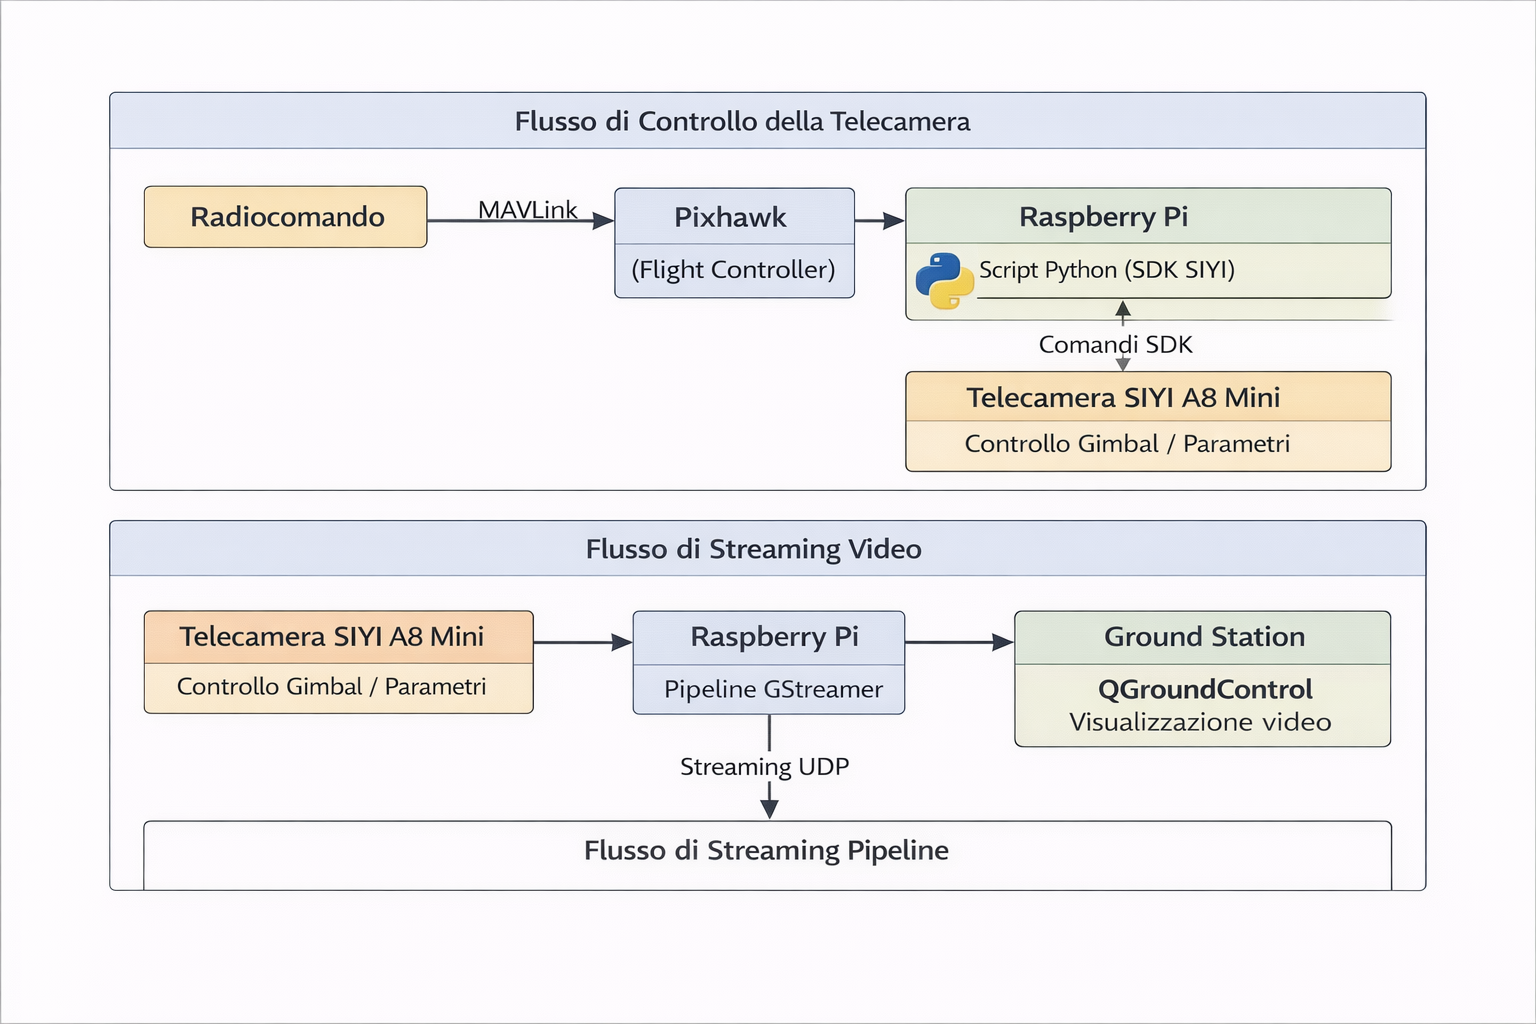
\includegraphics[width=0.8\textwidth]{schemaprogetto.png}
    \caption{Architettura del sistema di controllo e streaming video}
    \label{fig:architettura}
\end{figure}


\section{Ambito}
L’ambito di questo lavoro di tesi riguarda la progettazione e l’implementazione di un sistema per l’acquisizione, la trasmissione e il controllo remoto di un flusso video in tempo reale a bordo di un UAV multirotore. Il progetto è focalizzato sull’integrazione di una telecamera stabilizzata su gimbal con l’architettura di bordo del drone e con la stazione di terra, al fine di garantire una trasmissione video a bassa latenza e un controllo affidabile del sensore.\bigskip

Il lavoro si concentra sull’integrazione di componenti hardware e software commerciali, quali un Single Board Computer, un flight controller e una telecamera su gimbal, nonché sull’utilizzo e sull’ottimizzazione delle API messe a disposizione dal produttore della telecamera per migliorarne l’efficienza e l’affidabilità operativa.\bigskip

Dal punto di vista software, l’ambito del progetto comprende la gestione del flusso video in tempo reale, l’implementazione della pipeline di streaming verso la ground station e il controllo del gimbal tramite comandi provenienti dal radiocomando ed eseguiti a bordo del drone. La trasmissione del flusso video viene analizzata considerando i principali vincoli operativi dei sistemi UAV, quali latenza e stabilità della comunicazione.\bigskip

Non rientrano nell’ambito della tesi la progettazione meccanica del drone, lo sviluppo di algoritmi di visione artificiale o la modifica del firmware del flight controller.
\section{Obiettivi}
Il progetto di tirocinio si propone di sviluppare un sistema integrato per la gestione della telecamera SIYI A8 Mini montata sul drone Holybro X500, con particolare attenzione all’ottimizzazione dello streaming video e al controllo remoto del gimbal. Gli obiettivi principali del progetto sono:

Analisi delle architetture hardware e software: comprendere le caratteristiche e le interazioni tra il drone, la telecamera e le piattaforme software coinvolte, al fine di definire una base solida per l’integrazione del sistema.

Gestione ottimizzata dello streaming video: implementare un flusso video efficiente e stabile tramite GStreamer utilizzando il protocollo UDP multicast, garantendo qualità, latenza ridotta e affidabilità nella trasmissione verso la ground station.

Implementazione del controllo remoto del gimbal: sviluppare le funzionalità di controllo della telecamera attraverso il SIYI SDK, consentendo movimenti precisi e sincronizzati con le operazioni del drone.

Integrazione con QGroundControl: permettere il monitoraggio in tempo reale dello streaming video e dello stato del gimbal tramite la piattaforma QGroundControl, garantendo una gestione centralizzata e user-friendly del sistema.

In sintesi, il progetto mira a creare un’infrastruttura completa per la gestione della telecamera su drone, combinando controllo remoto, trasmissione video efficiente e monitoraggio centralizzato

\section{Risultati}
Il lavoro di tesi ha portato allo sviluppo e alla validazione di un sistema integrato per la gestione del payload video di un UAV, in grado di garantire lo streaming video in tempo reale a bassa latenza e il controllo remoto completo della telecamera stabilizzata. In particolare, è stato realizzato un flusso video stabile e reattivo basato su protocolli standard, insieme a un meccanismo di gestione dei comandi provenienti dal radiocomando, inoltrati al sistema di bordo per il controllo del gimbal e delle principali funzionalità della telecamera.

Sono stati inoltre sviluppati script in linguaggio Python basati sulle API esistenti, opportunamente adattate e ottimizzate per rispondere alle esigenze specifiche del progetto, migliorandone l’efficienza e l’affidabilità operativa. I risultati ottenuti confermano la fattibilità di un’architettura modulare e flessibile, integrata con la ground station per il monitoraggio in tempo reale, capace di offrire prestazioni adeguate a contesti applicativi di controllo e sorveglianza mediante piattaforme UAV.
\section{Sinossi}
Il presente lavoro si concentra sull’ottimizzazione della trasmissione video a bassa latenza e sulla garanzia di una comunicazione affidabile tra il sistema di bordo e la stazione di terra, aspetti fondamentali per numerose applicazioni UAV, tra cui il monitoraggio ambientale, le ispezioni industriali e le operazioni di sorveglianza. La capacità di trasmettere immagini in tempo reale e di controllare i sensori a distanza è cruciale per garantire efficacia, sicurezza e tempestività delle operazioni sul campo.\bigskip

La soluzione proposta si basa sull’integrazione delle API fornite dal produttore della telecamera, consentendo il controllo remoto del gimbal. Questo viene comandato anche tramite radiocomando, utilizzando canali propriamente configurati per svolgere le varie funzioni. Parallelamente, è stata sviluppata una pipeline di streaming ad alte prestazioni tramite GStreamer, con trasmissione basata su protocollo UDP multicast, progettata per ridurre la latenza e massimizzare l’efficienza del flusso video verso la stazione di terra. L’architettura modulare adottata permette di adattare facilmente il sistema a diversi scenari operativi e configurazioni hardware.\bigskip

I risultati sperimentali confermano la fattibilità di un approccio modulare e flessibile, capace di garantire uno streaming video stabile, affidabile e a bassa latenza, unitamente a un controllo preciso e sicuro del sistema di acquisizione, sia via API sia tramite radiocomando. Tali caratteristiche permettono un monitoraggio in tempo reale altamente performante, supportando decisioni rapide e informate durante le missioni UAV. L’analisi evidenzia come l’architettura proposta possa rappresentare una soluzione efficace per scenari in cui la tempestività della comunicazione e la qualità del segnale video sono requisiti fondamentali.


\chapter{Il problema}
\label{cap:problema}
\newpage



\section{Esposizione del problema affrontato}

L’impiego di sistemi UAV (Unmanned Aerial Vehicle) in contesti applicativi quali il monitoraggio ambientale, le ispezioni tecniche, la sorveglianza e il supporto operativo richiede sempre più frequentemente la disponibilità di sistemi di acquisizione video in tempo reale affidabili, flessibili e facilmente controllabili dall’operatore. In tali scenari, il flusso video rappresenta una delle principali fonti informative a supporto delle decisioni operative e deve pertanto essere trasmesso alla stazione di terra con una latenza ridotta e una qualità adeguata, al fine di consentire un controllo efficace durante le fasi di volo.

Uno dei principali problemi affrontati in questo progetto riguarda l’integrazione di un sistema di streaming video a bordo del drone in grado di operare in tempo reale senza compromettere la stabilità e la sicurezza del volo. Le piattaforme UAV sono infatti caratterizzate da vincoli stringenti in termini di risorse computazionali disponibili, consumo energetico e capacità di comunicazione, che rendono complessa la gestione simultanea delle operazioni di acquisizione, elaborazione, compressione e trasmissione del flusso video. Una progettazione non adeguata di tali funzionalità può introdurre ritardi, instabilità o interferenze con i sistemi critici di bordo.

Un’ulteriore criticità è rappresentata dalla necessità di controllare attivamente la telecamera durante il volo. In molte applicazioni operative, non è sufficiente ricevere un flusso video statico, ma risulta fondamentale poter modificare dinamicamente l’inquadratura mediante il controllo del gimbal, ad esempio per seguire un soggetto in movimento o focalizzarsi su specifiche aree di interesse. Tale controllo deve avvenire in modo intuitivo, reattivo e proporzionale ai comandi dell’operatore, tipicamente impartiti tramite radiocomando, garantendo una risposta fluida e priva di ritardi percepibili.

Dal punto di vista architetturale, il sistema si basa sull’interazione coordinata tra componenti eterogenee, tra cui un flight controller dedicato alla gestione del volo, un Single Board Computer incaricato dell’elaborazione e della gestione del flusso video, e una telecamera stabilizzata su più assi. La comunicazione tra questi elementi deve essere progettata con particolare attenzione, in modo da evitare interferenze con i loop di controllo del volo, che richiedono elevata affidabilità e tempi di risposta molto ridotti per garantire la sicurezza operativa.

Il problema affrontato in questo lavoro di tesi consiste quindi nella progettazione e realizzazione di una soluzione integrata che consenta l’acquisizione e la trasmissione di un flusso video in tempo reale, unitamente al controllo remoto della telecamera, mantenendo stabilità operativa, affidabilità del sistema e compatibilità con i vincoli tipici di una piattaforma UAV. L’obiettivo è dimostrare la possibilità di integrare tali funzionalità in un’unica architettura coerente, efficiente e utilizzabile in contesti operativi reali.

\section{Stato dell'arte}

Negli UAV di ultima generazione, l’impiego di telecamere stabilizzate su gimbal rappresenta un elemento chiave per applicazioni di monitoraggio, ispezione e ricognizione. La possibilità di acquisire immagini stabili e di alta qualità, unite alla trasmissione del flusso video in tempo reale verso una ground station, costituisce un requisito fondamentale in numerosi scenari operativi.

Sul mercato sono disponibili diversi payload professionali sviluppati da produttori affermati come DJI, Gremsy e Siyi, che offrono soluzioni integrate caratterizzate da elevate prestazioni, stabilizzazione avanzata su più assi e funzionalità di controllo remoto. Tali sistemi risultano particolarmente affidabili e adatti a contesti professionali, ma spesso presentano costi elevati e un livello di integrazione software limitato, dovuto all’adozione di ecosistemi proprietari.

In questo contesto, la Siyi A8 Mini si colloca come una soluzione compatta e leggera, progettata per droni di piccole e medie dimensioni. La telecamera è dotata di stabilizzazione su tre assi, zoom ottico e supporto a interfacce di comunicazione standard quali Ethernet e UART. Un aspetto particolarmente rilevante è la disponibilità di una SDK ufficiale open source, che consente lo sviluppo di applicazioni personalizzate per il controllo del gimbal, la gestione delle funzionalità della camera e l’accesso al flusso video tramite software.

L’adozione di una SDK aperta permette l’integrazione della telecamera con piattaforme di elaborazione basate su sistemi operativi Linux, come nel caso di single board computer quali Raspberry Pi 4. Questo approccio favorisce la realizzazione di architetture modulari e flessibili, nelle quali la gestione del payload video può essere integrata con algoritmi di automazione e sistemi di controllo del volo, rendendo possibile l’estensione futura verso missioni autonome e applicazioni avanzate.

Rispetto a soluzioni più costose e completamente integrate, come le famiglie DJI Zenmuse, la A8 Mini rappresenta un compromesso efficace tra qualità dell’immagine, peso, costo e flessibilità software. Tuttavia, l’impiego di componenti commerciali e protocolli di comunicazione standard introduce anche alcune criticità, in particolare per quanto riguarda la stabilità e l’affidabilità della trasmissione del flusso video in tempo reale in contesti operativi complessi.



\section{Sviluppo ad-hoc}

\subsection{Analisi dei requisiti}
Il progetto ha come obiettivo la realizzazione di un sistema UAV in grado di acquisire, elaborare e trasmettere in tempo reale un flusso video durante il volo, garantendo al contempo il controllo remoto della telecamera e l’integrazione con il sistema di controllo del drone.


\subsection{Requisiti funzionali}

I requisiti funzionali descrivono le funzionalità che il sistema deve offrire per soddisfare gli obiettivi del progetto.

In particolare, il sistema deve:
\begin{itemize}
    \item acquisire un flusso video in tempo reale da una telecamera installata a bordo del drone;
    \item trasmettere il flusso video alla stazione di terra durante il volo;
    \item consentire il controllo remoto della telecamera tramite radiocomando;
    \item permettere il controllo del gimbal della telecamera (movimenti di pan e tilt) durante il volo;
    \item interpretare i comandi provenienti dal radiocomando e tradurli in azioni di controllo della telecamera;
    \item eseguire la logica di controllo della telecamera tramite software a bordo del drone;
    \item integrare il sistema di acquisizione e controllo video con il sistema di controllo del volo senza interferire con le funzioni di stabilizzazione e navigazione;
    \item operare in modo autonomo e continuo durante le fasi di volo.
\end{itemize}

Questi requisiti garantiscono che il sistema non si limiti alla sola acquisizione delle immagini, ma permetta un controllo dinamico e in tempo reale della telecamera da parte dell’operatore.

\subsection{Requisiti non funzionali}

I requisiti non funzionali definiscono le caratteristiche qualitative del sistema, influenzando in modo significativo le scelte progettuali e architetturali.

Il sistema deve:
\begin{itemize}
    \item garantire una latenza ridotta nella trasmissione del flusso video, rendendolo utilizzabile in tempo reale;
    \item assicurare un’elevata affidabilità operativa durante l’intera durata del volo;
    \item presentare un consumo energetico contenuto, compatibile con l’autonomia del drone;
    \item essere modulare e facilmente estendibile, consentendo l’aggiunta di nuove funzionalità software;
    \item mantenere una configurazione stabile e riproducibile;
    \item garantire una risposta fluida e immediata ai comandi di controllo della telecamera.
\end{itemize}

Tali requisiti sono particolarmente rilevanti in un contesto UAV, dove le risorse computazionali ed energetiche sono limitate e la stabilità del sistema rappresenta un fattore critico.

\subsection{Requisiti prestazionali}

I requisiti prestazionali definiscono i livelli minimi di prestazione che il sistema deve garantire per risultare efficace nel contesto operativo previsto.

In particolare:
\begin{itemize}
    \item il flusso video deve mantenere una qualità sufficiente a consentire una chiara interpretazione delle immagini;
    \item la trasmissione del flusso video deve risultare stabile e continua, evitando interruzioni significative;
    \item il sistema deve essere in grado di elaborare e inoltrare il flusso video senza compromettere le altre funzionalità di bordo;
    \item il tempo di risposta ai comandi impartiti tramite radiocomando deve essere compatibile con un utilizzo in tempo reale;
    \item i movimenti del gimbal devono risultare fluidi e proporzionali ai comandi dell’operatore.
\end{itemize}

Anche in assenza di metriche numeriche stringenti, questi requisiti permettono di valutare l’efficacia della soluzione implementata.



\subsection{Modello di sviluppo}


Lo sviluppo del sistema è stato condotto seguendo un approccio iterativo e incrementale, ritenuto particolarmente adatto alla natura del progetto e al contesto applicativo UAV.  
Questo modello di sviluppo ha permesso di affrontare in modo progressivo le diverse problematiche, verificando a ogni fase il corretto funzionamento delle singole componenti prima di procedere all’integrazione completa del sistema.

L’intero processo di sviluppo è stato suddiviso in fasi successive, ciascuna delle quali ha avuto come obiettivo la risoluzione di specifici problemi tecnici e l’introduzione graduale di nuove funzionalità.

\subsubsection{Fase iniziale: sviluppo e stabilizzazione dello streaming video}

La prima fase dello sviluppo si è concentrata sulla risoluzione delle problematiche legate allo streaming video in tempo reale.  
In particolare, l’obiettivo iniziale era garantire l’acquisizione e la trasmissione stabile del flusso video prodotto dalla telecamera di bordo, minimizzando latenza e interruzioni.

In questa fase sono stati effettuati diversi test e configurazioni utilizzando strumenti dedicati allo streaming video, come GStreamer, al fine di analizzare il comportamento del flusso RTSP, valutare le prestazioni dei codec disponibili e individuare la configurazione più adatta al contesto embedded.  
Questa fase preliminare è risultata fondamentale per comprendere i limiti del sistema e per definire una base stabile su cui costruire le successive funzionalità.

\subsubsection{Sviluppo del controllo della telecamera tramite API e script Python}

Una volta ottenuto uno streaming video stabile, lo sviluppo si è concentrato sul controllo della telecamera.  
In questa fase sono stati studiati e utilizzati i meccanismi di controllo messi a disposizione dal produttore della telecamera, con particolare attenzione all’uso delle API dedicate.

Sono stati quindi sviluppati script in linguaggio Python, eseguiti direttamente sul Single Board Computer di bordo, con il compito di inviare comandi di controllo alla telecamera e di gestire i movimenti del gimbal.  
Questa fase ha permesso di implementare il controllo programmato delle funzionalità principali della telecamera, costituendo il collegamento tra i comandi esterni e il comportamento del dispositivo.

\subsubsection{Integrazione dello streaming video con la ground station}

Dopo aver implementato il controllo della telecamera e verificato il corretto funzionamento degli script software, lo sviluppo si è focalizzato sull’integrazione del flusso video con la ground station.  
In particolare, è stata implementata la trasmissione del flusso video verso QGroundControl, consentendo la visualizzazione in tempo reale delle immagini durante il volo.

Questa fase ha richiesto un’ulteriore attività di configurazione e test, al fine di garantire la compatibilità del flusso video con il software di ground control e di mantenere una trasmissione stabile e continua.

\subsubsection{Configurazione del radiocomando}

Successivamente, lo sviluppo si è concentrato sulla configurazione del radiocomando.  
In questa fase sono stati associati i diversi pulsanti e le leve del radiocomando alle specifiche funzioni della telecamera, definendo una mappatura coerente e intuitiva dei comandi.

L’obiettivo di questa fase era consentire all’operatore di controllare la telecamera in modo diretto e immediato, utilizzando il radiocomando come interfaccia principale durante il volo.  
La corretta configurazione del radiocomando ha rappresentato un passaggio fondamentale per l’integrazione completa del sistema di controllo.

\subsubsection{Test finali e validazione in volo}

L’ultima fase dello sviluppo è stata dedicata ai test finali e alla validazione del sistema in condizioni operative reali.  
Sono state effettuate prove di volo finalizzate a verificare il funzionamento simultaneo di tutte le componenti del sistema, inclusi lo streaming video, il controllo della telecamera e l’interazione con il sistema di controllo del volo.

I test di volo hanno permesso di confermare la stabilità del sistema, la corretta risposta ai comandi impartiti tramite radiocomando e l’assenza di interferenze con le funzioni di stabilizzazione del drone.  
Questa fase conclusiva ha consentito di validare l’intero processo di sviluppo e di dimostrare l’efficacia dell’approccio adottato.

\begin{figure}[h]
    \centering
    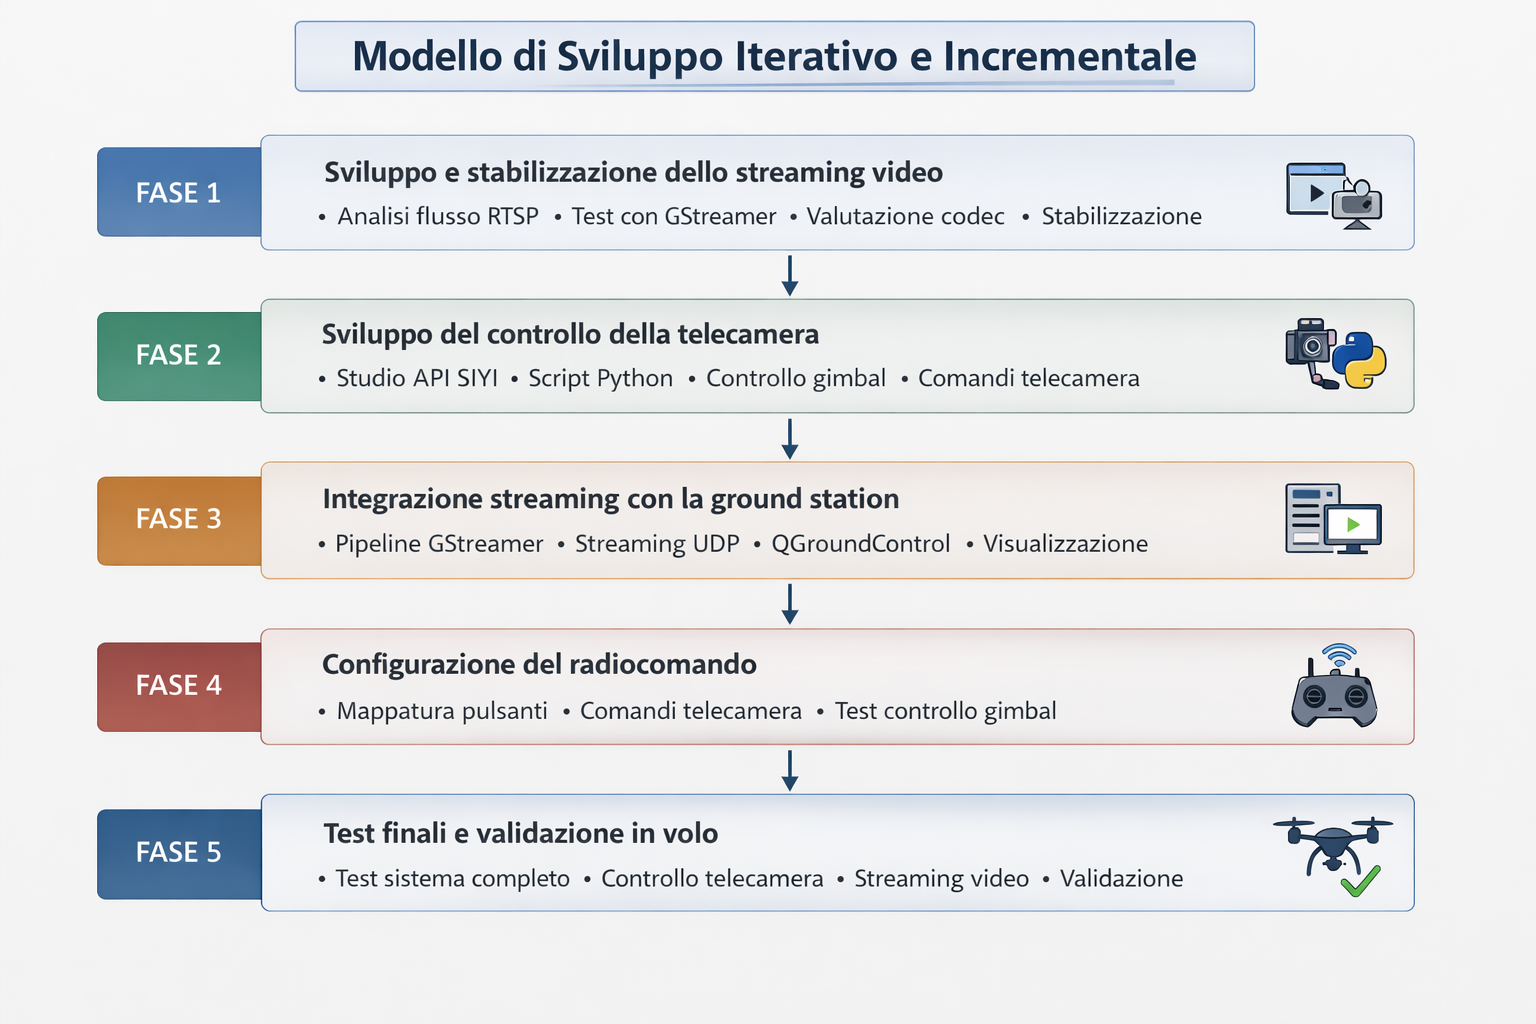
\includegraphics[width=0.8\textwidth]{schemasviluppo.png}
        \caption{Modello Di Sviluppo}
    \label{fig:architettura}
\end{figure}


\subsection{Architettura della soluzione}
L’architettura hardware del sistema è stata progettata con l’obiettivo di garantire un’elaborazione efficiente dei dati a bordo del drone, una trasmissione video in tempo reale stabile e un’elevata affidabilità operativa durante il volo. La soluzione si basa su una struttura modulare composta da un Single Board Computer, una telecamera stabilizzata, un flight controller, un radiocomando e un telaio dedicato per applicazioni UAV.

\subsubsection{Single Board Computer: Raspberry Pi 4}

Il \textbf{Raspberry Pi 4}\cite{raspberry_hw, raspberry_os} costituisce il nucleo computazionale del sistema, responsabile dell’elaborazione dei dati a bordo del drone. In particolare, il Single Board Computer (SBC) gestisce le seguenti funzioni principali:
\begin{itemize}
    \item Elaborazione delle immagini acquisite dalla telecamera;
    \item Gestione dei comandi diretti alla telecamera provenienti dal flight controller che li riceve dal radiocomando;
    \item Inoltro del flusso video in tempo reale verso la \textbf{ground station}.
\end{itemize}

Le principali specifiche tecniche del Raspberry Pi 4 utilizzato nel progetto sono:
\begin{itemize}
    \item \textbf{CPU}: ARM Cortex-A72 quad-core a 1.5 GHz
    \item \textbf{RAM}: 4 GB LPDDR4
    \item \textbf{Connettività}: Gigabit Ethernet, Wi-Fi 802.11ac
    \item \textbf{Sistema operativo}: Raspberry Pi OS Lite (modalità headless)
    \item \textbf{Consumo energetico medio}: circa 4.5 W
\end{itemize}

La scelta di un sistema operativo in modalità headless permette di ridurre il carico computazionale e i consumi energetici, rendendo il Raspberry Pi 4 particolarmente adatto a sistemi embedded destinati all’impiego su UAV.

\subsubsection{Sistema di acquisizione video: Telecamera SIYI A8 Mini}

La \textbf{SIYI A8 Mini}\cite{siyi_manual} rappresenta il componente principale per l’acquisizione video. Si tratta di una \textbf{gimbal camera stabilizzata su tre assi}, progettata per l’integrazione in sistemi UAV grazie alle dimensioni compatte e al peso ridotto.

Le principali caratteristiche tecniche della telecamera sono:
\begin{itemize}
    \item \textbf{Sensore}: CMOS da 12 MP
    \item \textbf{Output video}: RTSP, HDMI, CVBS
    \item \textbf{Risoluzioni supportate}: 720p (scelto per la soluzione) e 1080p
    \item \textbf{Codec video}: H.264 (scelto per la soluzione) e H.265 
    \item \textbf{Interfacce di controllo}: seriale ed Ethernet
\end{itemize}

La telecamera dispone di tre modalità di uscita video:
\begin{itemize}
    \item \textbf{micro-HDMI}: uscita digitale diretta via cavo
    \item \textbf{CVBS}: principalmente per sistemi FPV analogici
    \item \textbf{Ethernet (IP)}: genera un flusso video RTSP (Real Time Streaming Protocol)
\end{itemize}

Per questo progetto è stata selezionata l’uscita \textbf{RTSP su Ethernet}, in quanto consente l’inoltro efficiente del flusso video nella rete di bordo e verso la ground station.  

Considerando i requisiti di stabilità dello streaming in tempo reale e di efficienza energetica, la configurazione adottata prevede una risoluzione di \textbf{720p} con compressione \textbf{H.264}, garantendo un compromesso ottimale tra qualità video e carico computazionale.

\subsubsection{Flight Controller: Pixhawk 6X}

Il \textbf{Pixhawk 6X} \cite{px6} rappresenta il cuore del sistema di controllo del drone, gestendo tutti gli aspetti del volo, dalla stabilizzazione alla risposta ai comandi, grazie all’elaborazione dei dati provenienti dai sensori di bordo tramite algoritmi avanzati.  

Il dispositivo utilizza il \textbf{firmware ArduPilot}\cite{ardupilot} e comunica con il \textbf{Raspberry Pi} di bordo tramite connessione \textbf{UART}, consentendo l’integrazione di sistemi di telemetria, video e controllo avanzato.  

\textbf{Caratteristiche principali:}
\begin{itemize}
    \item Loop di stabilizzazione fino a 8 kHz
    \item Supporto a protocolli: DroneCAN, MAVLink, SBUS e PPM
    \item Interfacce multiple: Ethernet, UART, I2C, SPI e CAN bus
\end{itemize}

Il Pixhawk 6X è dotato di \textbf{tre IMU (Inertial Measurement Unit)}, ciascuna con i seguenti sensori:
\begin{itemize}
    \item \textbf{Accelerometro}: misura le accelerazioni lungo gli assi X, Y e Z
    \item \textbf{Giroscopio}: misura le velocità angolari sugli assi di roll, pitch e yaw
    \item \textbf{Magnetometro}: determina l’orientamento rispetto al nord magnetico
    \item \textbf{Barometro}: stima l’altitudine tramite la pressione atmosferica
\end{itemize}

I dati delle IMU vengono elaborati in tempo reale dal Pixhawk per regolare i motori e garantire un volo stabile, preciso e sicuro.

\subsubsection{Sistema di controllo remoto: RadioMaster Zorro}

Il \textbf{RadioMaster Zorro}\cite{radiomaster_zorro} costituisce il sistema di controllo remoto del drone e del gimbal, basato sul \textbf{firmware EdgeTX}, noto per l’elevato grado di personalizzazione e flessibilità.

\textbf{Caratteristiche principali:}
\begin{itemize}
    \item Supporto fino a 16 canali, per gestire simultaneamente tutte le funzioni del drone e del gimbal
    \item Raggio operativo fino a circa 1 km, variabile in base all’antenna e alle condizioni ambientali
    \item Display LCD retroilluminato, utile per monitorare i valori dei canali e informazioni operative anche in condizioni di scarsa illuminazione
    \item Alimentazione tramite batteria interna agli ioni di litio, garantendo lunga autonomia
\end{itemize}

Grazie alla configurazione dei canali personalizzata, il radiocomando permette di gestire con precisione sia i comandi di volo sia il controllo del gimbal, integrandosi perfettamente con la pipeline di controllo remoto sviluppata.

\subsubsection{ Struttura meccanica: Telaio Holybro X500}

Il telaio Holybro X500 costituisce la base strutturale del drone. È realizzato secondo una configurazione a quadricottero con una wheelbase di 500 mm ed è costruito in fibra di carbonio, materiale che garantisce un ottimo compromesso tra leggerezza e resistenza meccanica.

Il telaio ha un peso di circa 650 g ed è progettato per essere compatibile con un’ampia gamma di motori ed eliche. Il design modulare semplifica le operazioni di manutenzione e consente l’installazione agevole di componenti aggiuntivi, rendendolo particolarmente adatto a progetti sperimentali e applicazioni di ricerca in ambito UAV.



\chapter{Implementazione}
\label{cap:implementazione}
\newpage

\section{Descrizione dell'implementazione}
\bigskip
\noindent \textbf{Streaming del flusso video tramite GStreamer}
\bigskip
\noindent \textbf{Streaming del flusso video tramite GStreamer}
\bigskip

Una delle problematiche principali affrontate nello sviluppo del sistema riguarda la gestione dello streaming video in tempo reale dalla telecamera installata a bordo del drone verso la stazione di terra.
La possibilità di visualizzare il flusso video durante il volo rappresenta un requisito fondamentale per il corretto utilizzo operativo del sistema, in quanto consente all’operatore di monitorare l’ambiente circostante e di controllare attivamente l’inquadratura della telecamera, supportando decisioni rapide e consapevoli durante le fasi di missione.

Il sistema è stato configurato per ricevere dalla telecamera SIYI A8 Mini un flusso video in tempo reale tramite protocollo RTSP (Real Time Streaming Protocol).\cite{rtsp}
Il flusso video viene fornito dalla telecamera in risoluzione 720p ed è codificato utilizzando il codec H.264.
Questa scelta è stata effettuata tenendo conto delle limitazioni hardware tipiche di una piattaforma UAV e del Single Board Computer utilizzato.
Il codec H.264 offre infatti un buon compromesso tra qualità dell’immagine, stabilità del flusso e carico computazionale, risultando particolarmente adatto a scenari di streaming in tempo reale su sistemi embedded.
Inoltre, essendo uno standard ampiamente diffuso e consolidato, garantisce un’elevata compatibilità con i principali software di visualizzazione utilizzati nelle ground station, come QGroundControl e VLC.

Il flusso RTSP viene acquisito dal Raspberry Pi~4, che svolge il ruolo di nodo centrale per la gestione del video.
Il Raspberry Pi non si limita alla semplice ricezione del flusso, ma si occupa anche della sua riorganizzazione e del successivo inoltro verso la rete utilizzata dalla stazione di terra.
In questo modo, il Single Board Computer agisce come un vero e proprio ponte di rete, separando la rete Ethernet dedicata alla telecamera dalla rete WiFi impiegata per la comunicazione con la ground station, senza interferire con le funzionalità critiche di controllo del volo.

Una volta acquisito, il flusso video viene inoltrato utilizzando il protocollo UDP in modalità multicast sulla porta 5600.
La scelta del protocollo UDP è stata dettata dalle esigenze di riduzione della latenza e di maggiore reattività del flusso video.
A differenza del protocollo TCP, l’UDP non implementa meccanismi di ritrasmissione dei pacchetti persi, evitando così ritardi aggiuntivi dovuti alla gestione degli errori di trasmissione.
Questo approccio risulta particolarmente indicato per applicazioni di streaming in tempo reale, dove la tempestività delle informazioni è più importante della perfetta integrità di ogni singolo frame.

L’uso della modalità multicast consente di rendere il flusso video accessibile simultaneamente a più client presenti sulla stessa rete.
In questo modo, applicazioni come QGroundControl e media player come VLC possono visualizzare lo stesso flusso video senza la necessità di creare connessioni separate.
Questo approccio riduce il carico computazionale sul Raspberry Pi e migliora l’efficienza complessiva del sistema, evitando la duplicazione dei flussi video e semplificando la scalabilità dell’architettura.

Durante le fasi di test, il sistema ha mostrato una latenza end-to-end mediamente inferiore ai 500~ms.
Tale valore è risultato compatibile con i requisiti di controllo remoto della telecamera e ha consentito un utilizzo fluido e reattivo del sistema durante le operazioni di volo.
Anche in presenza di occasionali perdite di pacchetti, il flusso video si è mantenuto stabile e utilizzabile, confermando l’adeguatezza delle scelte progettuali adottate.

Per la gestione del flusso video è stato utilizzato GStreamer\cite{gstreamer}, un framework multimediale modulare ampiamente diffuso in ambito embedded e professionale.
GStreamer consente la costruzione di pipeline personalizzate per l’acquisizione, l’elaborazione e la trasmissione di flussi audio e video.
Grazie alla sua architettura modulare basata su elementi concatenabili, è possibile adattare in modo fine il comportamento del sistema alle esigenze specifiche del progetto, privilegiando ad esempio la riduzione della latenza rispetto alla qualità visiva.

Prima di poter utilizzare GStreamer, è stato necessario installare i pacchetti software richiesti.
L’installazione avviene tramite il seguente comando:

\begin{verbatim}
sudo apt install gstreamer1.0-tools gstreamer1.0-plugins-base \
gstreamer1.0-plugins-good gstreamer1.0-plugins-bad \
gstreamer1.0-plugins-ugly
\end{verbatim}

Questi pacchetti forniscono il supporto ai principali formati multimediali e ai protocolli necessari per la gestione del flusso RTSP e della trasmissione RTP su UDP, garantendo la disponibilità degli elementi richiesti dalla pipeline implementata.

Il flusso video RTSP viene fornito dalla telecamera all’endpoint:

\begin{verbatim}
rtsp://192.168.144.25:8554/main.264
\end{verbatim}

Una volta individuato l’endpoint corretto, è stata definita una pipeline GStreamer in grado di ricevere il flusso RTSP, estrarre i pacchetti RTP contenenti il video H.264 e inoltrarli sulla rete locale in modalità multicast.
La pipeline utilizzata è la seguente:

\begin{verbatim}
gst-launch-1.0 -v rtspsrc location=rtsp://192.168.144.25:8554/main.264 \
latency=0 ! rtph264depay ! h264parse ! \
rtph264pay config-interval=1 pt=96 ! \
udpsink host=239.255.42.99 port=5600 auto-multicast=true ttl=1 sync=false
\end{verbatim}

L’elemento \texttt{rtspsrc} si occupa di stabilire la connessione RTSP con la telecamera e di ricevere il flusso video.  
Il parametro \texttt{latency=0} è stato impostato per ridurre al minimo il buffering interno introdotto dal jitter buffer di GStreamer, contribuendo a diminuire la latenza complessiva del sistema anche a costo di una maggiore sensibilità alle condizioni della rete.

Gli elementi \texttt{rtph264depay} e \texttt{h264parse} permettono rispettivamente di:  
\begin{itemize}
    \item estrarre il flusso H.264 dai pacchetti RTP;
    \item analizzare il flusso per individuare correttamente i frame e le informazioni di sincronizzazione necessarie alle fasi successive.
\end{itemize}

Il flusso viene quindi nuovamente incapsulato tramite \texttt{rtph264pay}, che suddivide il video in pacchetti RTP pronti per la trasmissione.  
\begin{itemize}
    \item Il parametro \texttt{config-interval=1} assicura che le informazioni di configurazione vengano trasmesse periodicamente, facilitando una rapida sincronizzazione da parte dei client riceventi.
    \item Il parametro \texttt{pt=96} specifica il tipo di payload nei pacchetti RTP.
\end{itemize}

L’invio del flusso sulla rete locale avviene tramite l’elemento \texttt{udpsink}.  
\begin{itemize}
    \item \texttt{auto-multicast=true} abilita automaticamente la modalità multicast senza la necessità di configurazioni manuali aggiuntive.
    \item \texttt{ttl=1} limita la propagazione dei pacchetti alla sola rete locale, evitando un inoltro indesiderato del traffico video su reti esterne.
    \item \texttt{sync=false} disabilita la sincronizzazione temporale con il clock di sistema, permettendo l’inoltro immediato dei pacchetti e riducendo ulteriormente la latenza end-to-end del flusso video.
\end{itemize}

È opportuno sottolineare che, sebbene la modalità multicast consenta una distribuzione efficiente del flusso a più dispositivi, in scenari con un singolo client è possibile configurare il sistema in modalità unicast.  
Tale soluzione può migliorare la qualità visiva del flusso e ridurre la perdita di pacchetti, sacrificando però la possibilità di visualizzazione simultanea su più dispositivi.
\bigskip

\subsection{Valutazione delle prestazioni della pipeline GStreamer}

La pipeline GStreamer implementata è stata sottoposta a una serie di test mirati a valutare la stabilità del flusso video, la latenza end-to-end e l’impatto sulle risorse del Raspberry Pi 4.  
Tali valutazioni hanno permesso di verificare se la configurazione scelta, comprensiva del codec H.264 e della trasmissione UDP multicast, soddisfacesse i requisiti di reattività e affidabilità necessari per il controllo remoto della telecamera a bordo del drone.

Per la valutazione sono stati considerati i seguenti parametri:
\begin{itemize}
    \item \textbf{Risoluzione del flusso video}: il sistema è stato testato principalmente a 720p, scelta motivata dal compromesso tra qualità visiva e latenza. Tentativi di utilizzo della risoluzione 1080p hanno evidenziato un incremento significativo della latenza.
    \item \textbf{Codec video}: H.264 è stato confermato come la soluzione più adatta, in quanto riduce il carico computazionale rispetto a H.265, garantendo compatibilità con QGroundControl, VLC e altri client.
    \item \textbf{Latenza end-to-end}: misurazioni effettuate durante i test hanno evidenziato valori medi di circa 300 ms a 720p. La latenza a 1080p salirebbe fino a circa 900 ms, rendendo il flusso meno adatto a scenari con esigenze di reattività immediata.
    \item \textbf{Consumo di CPU sul Raspberry Pi}: il flusso a 720p con H.264 ha comportato un utilizzo medio della CPU del 28\%, mentre a 1080p la CPU ha raggiunto picchi del 65\%, riducendo la capacità del sistema di eseguire simultaneamente altri compiti come il controllo del gimbal tramite Pymavlink e SIYI SDK.
\end{itemize}

In aggiunta, la pipeline è stata avviata tramite un servizio \texttt{systemd}, che include un ritardo predefinito di 10 secondi (\texttt{ExecStartPre=/bin/sleep 10}) per garantire che la configurazione della rete Ethernet fosse completata prima dell’inizio dello streaming. Questo accorgimento ha permesso di ottenere un avvio affidabile della pipeline senza corruzione dei frame o interruzioni del flusso video.

I test hanno quindi confermato che:
\begin{itemize}
    \item la pipeline GStreamer fornisce uno streaming stabile e a bassa latenza a 720p;
    \item la modalità multicast consente la visualizzazione simultanea su più client senza appesantire ulteriormente il Raspberry Pi;
    \item il bilanciamento tra qualità del video e utilizzo delle risorse è adeguato per scenari operativi di UAV.
\end{itemize}

Questi risultati hanno rappresentato un passo fondamentale per il raggiungimento degli obiettivi progettuali, garantendo all’operatore una visione affidabile e reattiva dell’ambiente circostante durante le missioni di volo.

\subsection{Diagnosi e risoluzione dei problemi di rete Ethernet}

Durante le prime fasi di test della pipeline GStreamer, è emerso un problema critico che ha compromesso la visibilità del flusso video sulla Ground Station.  
Il video appariva completamente verde e distorto, segno evidente di corruzione dei frame ricevuti, rendendo lo streaming inutilizzabile.  
Questo comportamento anomalo ha reso necessario un approfondimento delle cause alla base del malfunzionamento.

\subsubsection{Analisi del problema}

L’analisi tecnica \cite{forum_siyi} ha evidenziato che il problema non risiedeva nella logica della pipeline GStreamer, né nella configurazione del flusso RTSP, ma nello strato fisico della connessione Ethernet tra il Raspberry Pi 4 e la telecamera Siyi A8 Mini.  

La causa principale è stata identificata nella negoziazione automatica della velocità Ethernet. In condizioni ideali, i due dispositivi dovrebbero negoziare automaticamente la massima velocità supportata (100 Mbps nel nostro caso). Tuttavia, il chip PHY della telecamera Siyi, pur dichiarando compatibilità con i 100 Mbps, non era in grado di sostenere tale throughput in modo affidabile.  
Di conseguenza, il controller Ethernet Gigabit del Raspberry Pi inviava dati a una velocità superiore a quella gestibile dalla telecamera, causando:  

\begin{itemize}
    \item perdita di pacchetti durante lo streaming;
    \item errori CRC (Cyclic Redundancy Check) sui frame ricevuti;
    \item corruzione dei dati video e visualizzazione distorta sulla Ground Station.
\end{itemize}

Questo fenomeno è tipico di situazioni in cui la rete Ethernet non riesce a gestire correttamente il jitter e il buffering dei pacchetti, risultando particolarmente critico in scenari di streaming video in tempo reale a bassa latenza.

\subsubsection{Soluzione implementativa}

Per risolvere il problema è stata adottata una strategia di modifica manuale della velocità di connessione tramite il comando \texttt{ethtool} sul Raspberry Pi.  
La connessione è stata bloccata a 10 Mbps full-duplex, disabilitando l’autonegoziazione automatica, con il seguente comando:

\begin{verbatim}
sudo ethtool -s eth0 speed 10 duplex full autoneg off
\end{verbatim}

\noindent I parametri del comando hanno il seguente significato:
\begin{itemize}
    \item \texttt{speed 10}: imposta la velocità della porta Ethernet a 10 Mbps;
    \item \texttt{duplex full}: abilita la trasmissione e la ricezione simultanea dei dati;
    \item \texttt{autoneg off}: disabilita l’autonegoziazione automatica, evitando tentativi falliti di sincronizzazione a velocità superiori.
\end{itemize}

Questa configurazione ha ridotto drasticamente la perdita di pacchetti e gli errori di CRC, garantendo uno streaming H.264 stabile e privo di corruzioni a 720p.  
Sebbene la velocità massima sia inferiore ai 100 Mbps teorici, essa risulta sufficiente per sostenere il flusso video codificato in H.264 a risoluzione 720p, con bassa latenza e senza compromettere l’esperienza utente.



Per garantire che questa configurazione venisse applicata automaticamente ad ogni avvio del drone, sono stati creati due servizi \texttt{systemd} sul Raspberry Pi:

\begin{itemize}
    \item \texttt{ethernet-speed.service}: esegue automaticamente il comando \texttt{ethtool} appena l’interfaccia di rete è attiva, assicurando la corretta velocità di connessione prima dell’avvio dello streaming;
    \item \texttt{streaming.service}: avvia automaticamente la pipeline GStreamer per l’inoltro del flusso video in modalità multicast.
\end{itemize}

Questa strategia garantisce che lo streaming video sia affidabile e disponibile immediatamente dopo l’accensione del drone, senza necessità di interventi manuali da parte dell’operatore.

\subsubsection{Osservazioni pratiche e test}

Durante le fasi di validazione, l’adozione della velocità forzata ha permesso di ottenere:  

\begin{itemize}
    \item stabilità del flusso video anche in scenari con più client connessi in multicast;
    \item latenza end-to-end inferiore ai 500 ms, compatibile con il controllo remoto della telecamera;
    \item assenza di artefatti visivi causati da pacchetti corrotti o frame persi.
\end{itemize}

Questa esperienza ha evidenziato come, in sistemi embedded e UAV, sia fondamentale considerare non solo la logica software, ma anche le caratteristiche hardware della rete, la gestione del jitter e la compatibilità tra dispositivi per garantire streaming affidabili e performanti.

\noindent 

\bigskip

\subsection{Controllo remoto del gimbal tramite radiocomando}

Il controllo remoto del gimbal della telecamera costituisce una componente essenziale del sistema sviluppato, in quanto consente all’operatore di modificare dinamicamente l’inquadratura durante il volo, adattandola al contesto operativo.  
A differenza di una semplice visualizzazione passiva del flusso video, il sistema realizzato permette un’interazione attiva e in tempo reale con il payload, migliorando significativamente l’efficacia delle operazioni di monitoraggio.

Per l’implementazione di tale funzionalità è stato utilizzato un radiocomando RadioMaster Zorro, dispositivo che mette a disposizione fino a 16 canali configurabili. Ogni canale può essere associato a un controllo fisico (stick, slider, levetta o pulsante), offrendo un’elevata flessibilità nella mappatura dei comandi.

\subsubsection{Architettura di comunicazione}

Dal punto di vista architetturale, il sistema è composto da tre elementi principali:

\begin{itemize}
    \item Il \textbf{radiocomando}, che genera i segnali di input dell’operatore;
    \item Il \textbf{Pixhawk}, che funge da flight controller e riceve i valori dei canali tramite il ricevitore radio;
    \item Il \textbf{Raspberry Pi}, collegato al Pixhawk tramite interfaccia UART, incaricato di interpretare i valori dei canali e tradurli in comandi per la telecamera.
\end{itemize}

Il Pixhawk aggiorna in tempo reale i valori dei canali ricevuti dal radiocomando e li rende disponibili attraverso il protocollo MAVLink\cite{mavlink}.  
Il Raspberry Pi, utilizzando la libreria PyMAVLink, interroga periodicamente il flight controller per leggere i valori dei canali di interesse.

Questa soluzione consente di creare un vero e proprio “ponte software” tra il sistema di controllo del volo e il payload video, mantenendo separati i due sottosistemi dal punto di vista hardware ma coordinandoli a livello applicativo.

\subsubsection{Mappatura dei canali e logica di controllo}

Per il controllo del gimbal e delle funzioni principali della telecamera sono stati dedicati specifici canali ausiliari:

\begin{itemize}
    \item Due canali analogici per il controllo proporzionale degli assi di \textit{yaw} (imbardata) e \textit{pitch} (beccheggio) del gimbal;
    \item Due canali digitali per le funzioni di \textit{zoom in} e \textit{zoom out}.
\end{itemize}

I canali analogici forniscono valori proporzionali alla posizione del controllo fisico, consentendo un movimento fluido e continuo del gimbal.  
I canali digitali, invece, generano valori discreti che vengono interpretati come comandi di attivazione o disattivazione dello zoom.

Il firmware del Pixhawk normalizza tali valori in un intervallo tipico compreso tra 1000 e 2000, che il Raspberry Pi riconverte in un intervallo logico più adatto alla gestione applicativa. Questa fase di normalizzazione e traduzione è fondamentale per garantire un comportamento coerente e prevedibile del sistema.

\subsubsection{Implementazione software}

La logica di gestione dei comandi è implementata nel file \texttt{controller\_radio.py}, che rappresenta il modulo software responsabile dell’orchestrazione tra:

\begin{itemize}
    \item la lettura dei canali tramite PyMAVLink;
    \item l’elaborazione dei valori ricevuti;
    \item l’invio dei comandi alla telecamera tramite l’API Python della SIYI SDK.
\end{itemize}

Lo script opera in modo continuo, monitorando le variazioni dei canali configurati.  
Quando viene rilevata una variazione significativa rispetto allo stato precedente, il sistema genera il comando corrispondente per il gimbal o per lo zoom, inviandolo alla telecamera attraverso la connessione Ethernet.

Le API fornite su github \cite{siyi_sdk_repo} sono state opportunamente adattate e ottimizzate (come descritto nel capitolo successivo) per migliorare la reattività e ridurre il tempo di risposta ai comandi dell’operatore.

\subsubsection{Considerazioni sulle prestazioni}

I test effettuati hanno dimostrato che il tempo di risposta tra l’azione sul radiocomando e il movimento effettivo del gimbal è compatibile con l’utilizzo in scenari operativi reali.  
La comunicazione seriale tra Pixhawk e Raspberry Pi, unita alla trasmissione dei comandi via UDP verso la telecamera, introduce una latenza contenuta che non compromette la manovrabilità del sistema.

L’integrazione tra controllo del volo, streaming video e gestione del gimbal risulta quindi stabile e coerente, permettendo all’operatore di mantenere il pieno controllo del payload durante tutte le fasi della missione.

\bigskip
\noindent \textbf{Lettura dei canali RC dal Pixhawk}
\bigskip

Affinché il Raspberry Pi possa leggere i valori dei canali del radiocomando, è necessario richiedere esplicitamente al Pixhawk l’invio continuo di tali informazioni.
Questa operazione viene effettuata tramite protocollo MAVLink, utilizzando una connessione seriale sulla porta \texttt{/dev/ttyAMA0}.

Nel costruttore della classe principale dello script Python viene stabilita la connessione con il Pixhawk e viene richiesto l’invio periodico dei valori dei canali RC.
Il codice utilizzato è il seguente:

\begin{verbatim}
def __init__(self, connection="/dev/ttyAMA0", baud=57600,
             cam_ip="192.168.144.25", cam_port=37260):

    # Connessione al Pixhawk
    self.master = mavutil.mavlink_connection(connection, baud=baud)
    self.master.wait_heartbeat()
    print("Heartbeat ricevuto: connessione stabilita.")

    # Richiesta invio dei dati dei canali RC
    self.master.mav.request_data_stream_send(
        self.master.target_system,
        self.master.target_component,
        mavutil.mavlink.MAV_DATA_STREAM_RC_CHANNELS,
        20,  # frequenza di aggiornamento (Hz)
        1
    )
\end{verbatim}

Questo blocco svolge tre operazioni fondamentali:

\begin{itemize}
    \item stabilisce la connessione seriale con il Pixhawk e attende la ricezione dell’heartbeat, confermando che la comunicazione è attiva;
    \item richiede al flight controller l’invio continuo dei valori dei canali RC con una frequenza di aggiornamento pari a 20 Hz;
    \item inizializza la comunicazione UDP con la telecamera, creando l’oggetto che gestirà l’invio dei comandi tramite SIYI SDK.
\end{itemize}

\bigskip

\bigskip
\noindent \textbf{Lettura e interpretazione dei valori dei canali}
\bigskip

Una volta completata l’inizializzazione, lo script entra in un ciclo continuo nel quale vengono eseguite tre fasi principali: ascolto dei dati, interpretazione dei valori e invio dei comandi alla telecamera.
\begin{verbatim}
while True:

    # 1. ASCOLTO: ricezione messaggi RC_CHANNELS
    msg = self.master.recv_match(type='RC_CHANNELS',
                                 blocking=True, timeout=0.001)
    if not msg:
        continue

    # Estrazione dei canali di interesse
    rc_yaw_val = msg.chan12_raw
    rc_pitch_val = msg.chan11_raw
    zoom_in_pressed = msg.chan8_raw > 1700
    zoom_out_pressed = msg.chan9_raw > 1700

    # 2. TRADUZIONE: mappatura PWM (1000-2000) in angoli
    new_yaw = map_value(rc_yaw_val, 1000, 2000, -160, 160)
    new_pitch = map_value(rc_pitch_val, 1000, 2000, -135, 45)

    # 3. COMANDO: invio comandi alla telecamera
    self.cam.setGimbalRotation(new_yaw, new_pitch)

    if zoom_in_pressed and not zoom_out_pressed:
        self.cam.requestZoomIn()
    elif zoom_out_pressed and not zoom_in_pressed:
        self.cam.requestZoomOut()
    else:
        self.cam.requestZoomHold()
\end{verbatim}

\bigskip
\noindent
Durante la fase di ascolto, il Raspberry Pi riceve messaggi MAVLink di tipo \texttt{RC\_CHANNELS}, contenenti i valori grezzi dei canali del radiocomando, tipicamente compresi tra 1000 e 2000.

\medskip
\noindent
Nella fase di traduzione, tali valori vengono convertiti in grandezze utilizzabili dalla telecamera. In particolare:

\begin{itemize}
    \item il canale 12 viene utilizzato per il controllo dell’asse di \textit{yaw};
    \item il canale 11 per il controllo dell’asse di \textit{pitch};
    \item i canali 8 e 9 sono dedicati rispettivamente alle funzioni di \textit{zoom in} e \textit{zoom out}.
\end{itemize}

\medskip
\noindent
I valori PWM associati a yaw e pitch vengono mappati in intervalli angolari coerenti con le capacità meccaniche del gimbal.

\medskip
\noindent
Per quanto riguarda lo zoom, essendo controllato da pulsanti, non è necessario un valore proporzionale: viene utilizzata una soglia (ad esempio 1700) per determinare se il pulsante sia premuto o meno.

\medskip
\noindent
Infine, nella fase di comando, i valori elaborati vengono inviati alla telecamera tramite connessione UDP.

\medskip
\noindent
Il metodo \texttt{setGimbalRotation()} gestisce l’orientamento del gimbal, mentre le funzioni \texttt{requestZoomIn()}, \texttt{requestZoomOut()} e \texttt{requestZoomHold()} controllano lo stato dello zoom.

\medskip
\noindent
Questa architettura modulare, basata sulla separazione tra acquisizione dei dati, elaborazione e invio dei comandi, consente un controllo reattivo e continuo del payload, mantenendo chiara la distinzione tra logica di comunicazione MAVLink e gestione della telecamera tramite SDK dedicata.

\bigskip
\noindent \textbf
\bigskip

\section{Gestione multi-thread del controllo del payload}

\bigskip

La logica di controllo del gimbal e dello zoom non è stata implementata in un unico ciclo sequenziale,
poiché la funzione di lettura dei messaggi MAVLink

\begin{verbatim}
self.master.recv_match(type='RC_CHANNELS', blocking=True)
\end{verbatim}

è di natura bloccante.  
Ciò significa che l’esecuzione dello script rimane sospesa finché non viene ricevuto un nuovo messaggio dal Pixhawk.
In una struttura monolitica, questo comportamento introdurrebbe ritardi nell’invio dei comandi alla telecamera,
rendendo il movimento del gimbal meno fluido e lo zoom poco reattivo.

Per evitare questo problema, il sistema è stato progettato utilizzando più thread paralleli,
separando la fase di lettura dei dati dalla fase di esecuzione dei comandi.
In questo modo la ricezione dei valori RC non interferisce con l’invio dei comandi alla telecamera.

\bigskip
\section*{Gestione della rotazione del gimbal}

\bigskip

Per il controllo degli assi yaw e pitch sono stati utilizzati due thread distinti.

Il primo thread, denominato \textit{RC Position Writer}, ha il compito di leggere continuamente
i valori dei canali provenienti dal radiocomando.
Nel nostro caso, il canale 12 controlla il movimento orizzontale (yaw),
mentre il canale 11 controlla il movimento verticale (pitch).

\begin{verbatim}
msg = self.master.recv_match(type='RC_CHANNELS', blocking=True)

rc_yaw = msg.chan12_raw
rc_pitch = msg.chan11_raw
\end{verbatim}

Essendo i valori ricevuti segnali PWM grezzi compresi tra 1000 e 2000,
è necessario convertirli nell’intervallo angolare supportato dal gimbal.
A questo scopo viene utilizzata una funzione di mappatura lineare:

\begin{verbatim}
def map_rc_fast(self, rc_value, scale, offset):
    return rc_value * scale + offset
\end{verbatim}

I valori vengono quindi trasformati negli angoli effettivi:

\begin{verbatim}
new_yaw = self.map_rc_fast(rc_yaw, self.yaw_scale, self.yaw_offset)
new_pitch = self.map_rc_fast(rc_pitch, self.pitch_scale, self.pitch_offset)
\end{verbatim}

Il secondo thread, denominato \textit{Gimbal Executor}, si occupa dell’invio dei comandi alla telecamera.
Per evitare traffico di rete superfluo e ridurre il carico sul sistema,
il comando viene trasmesso solo quando viene rilevata una variazione rispetto all’ultima posizione inviata:

\begin{verbatim}
if new_yaw != self.target_yaw or new_pitch != self.target_pitch:
    self.cam.setGimbalRotation(new_yaw, new_pitch)
    print(f"YAW: {new_yaw} | PITCH: {new_pitch}")
\end{verbatim}

Questa separazione consente di aggiornare continuamente il valore target
senza mettere in coda comandi obsoleti.
Se l’operatore modifica rapidamente la posizione dello slider,
il sistema considera sempre e soltanto l’ultimo valore disponibile,
garantendo una risposta immediata e priva di inerzia percepibile.

\bigskip
\section*{Implementazione dello zoom}

\bigskip

Anche per la gestione dello zoom è stata adottata una struttura basata su due thread distinti:
uno dedicato alla lettura dello stato dei pulsanti,
l’altro all’invio dei comandi alla telecamera.

I pulsanti associati allo zoom generano un segnale digitale:
circa 2000 quando premuti e circa 1000 quando rilasciati.
Definendo una soglia pari a 1700 è possibile discriminare in modo affidabile
lo stato del comando.

\begin{verbatim}
self.zoom_in = msg.chan8_raw > 1700
self.zoom_out = msg.chan9_raw > 1700
\end{verbatim}

Il thread esecutore implementa una logica a tre stati:
zoom in, zoom out e arresto.

\begin{verbatim}
if self.zoom_in and not self.zoom_out:
    self.cam.requestZoomIn()
elif self.zoom_out and not self.zoom_in:
    self.cam.requestZoomOut()
else:
    self.cam.requestZoomHold()
\end{verbatim}

In questo modo, mantenendo premuto il pulsante lo zoom avanza o arretra in modo continuo,
mentre al rilascio viene inviato il comando di arresto.
La gestione separata dei thread impedisce che l’attivazione dello zoom interferisca
con il movimento del gimbal, mantenendo indipendenti le due funzionalità.

\bigskip


\bigskip

\bigskip
\section*{Vantaggi dell’architettura multi-thread}

\bigskip

\section*{Considerazioni sull’architettura concorrente}

\bigskip

L’implementazione del controllo mediante più thread paralleli
non rappresenta soltanto una scelta organizzativa del codice,
ma una decisione progettuale orientata alle prestazioni.

La separazione tra acquisizione dei dati RC ed esecuzione dei comandi
consente di eliminare i vincoli temporali tipici di un’architettura sequenziale.
In assenza di tale suddivisione, ogni operazione di lettura bloccante
introdurrebbe un ritardo cumulativo sull’intero ciclo di controllo,
con ripercussioni dirette sulla fluidità del movimento del gimbal.

Un primo effetto positivo riguarda la dinamica di risposta.
Gli assi yaw e pitch vengono aggiornati in modo continuo,
indipendentemente dallo stato dello zoom,
poiché le rispettive logiche operative non condividono lo stesso flusso esecutivo.
Questo isolamento funzionale impedisce interferenze reciproche
e mantiene costante la frequenza di aggiornamento percepita dall’operatore.

Un secondo aspetto rilevante è legato all’efficienza della comunicazione.
L’invio dei comandi alla telecamera avviene esclusivamente
quando si verifica una variazione significativa dello stato.
In questo modo si evita la generazione di traffico ridondante sulla rete UDP,
limitando il carico sia sul Raspberry Pi sia sul firmware della telecamera.

Infine, la struttura concorrente favorisce la manutenibilità del sistema.
La suddivisione delle responsabilità in unità logiche indipendenti
semplifica eventuali modifiche o ampliamenti futuri.
L’integrazione di nuove funzionalità può essere realizzata
introducendo ulteriori thread dedicati,
senza alterare l’equilibrio delle componenti già operative.

Nel complesso, l’architettura multi-thread non migliora soltanto la reattività,
ma contribuisce anche alla robustezza e alla scalabilità del sistema di controllo.

\bigskip
\noindent
Un esempio pratico evidenzia il vantaggio del disaccoppiamento tra lettura ed esecuzione.

Si consideri il caso in cui l’operatore sposti rapidamente lo slider dello yaw
verso un’estremità, generando un comando corrispondente a un angolo elevato,
e subito dopo lo riporti in posizione centrale.

Nel sistema implementato:

\begin{itemize}
    \item il thread di lettura aggiorna immediatamente il nuovo valore target;
    \item il thread esecutore invia il comando di rotazione corrispondente;
    \item se nel frattempo il valore cambia nuovamente, il target precedente viene semplicemente sovrascritto;
    \item al ciclo successivo, il thread esecutore invia direttamente l’ultimo valore disponibile.
\end{itemize}

Il risultato è che il gimbal non esegue una sequenza di comandi in coda,
ma reagisce sempre all’ultimo input valido.
Questo comportamento elimina ritardi accumulati e riduce la latenza percepita,
fornendo un controllo che risulta immediato all’operatore.

\bigskip
\section*{Avvio e supervisione dei thread}

\bigskip

La strategia multi-thread viene attivata all’interno della funzione principale
\texttt{run()}, responsabile della creazione e dell’avvio dei thread di controllo.

\begin{verbatim}
def run(self):

    threading.Thread(
        target=self.zoom_rc_reader_thread,
        daemon=True
    ).start()

    threading.Thread(
        target=self.zoom_executor_thread,
        daemon=True
    ).start()

    threading.Thread(
        target=self.rc_position_writer_thread,
        daemon=True
    ).start()

    threading.Thread(
        target=self.gimbal_executor_thread,
        daemon=True
    ).start()

    try:
        while True:
            time.sleep(0.0001)
    except KeyboardInterrupt:
        print("\nArresto controller...")
        self.running = False
        self.target_updated.set()
\end{verbatim}

All’interno di questa funzione vengono istanziati e avviati i quattro thread:
due dedicati al gimbal (lettura ed esecuzione) e due dedicati allo zoom.
Tutti vengono creati con il parametro \texttt{daemon=True},
il che implica che la loro esecuzione è subordinata al thread principale.

Il ciclo infinito contenente \texttt{time.sleep(0.0001)} non svolge operazioni di controllo,
ma ha lo scopo di mantenere attivo il processo principale
con un consumo di CPU trascurabile.
In questo modo le risorse computazionali vengono lasciate ai thread operativi,
che gestiscono effettivamente la logica di controllo.

L’interruzione manuale tramite \texttt{Ctrl+C} consente di uscire dal ciclo,
terminando in modo ordinato l’esecuzione durante le fasi di test o debug.\bigskip
\subsection{Visualizzazione del flusso video su QGroundControl}
\bigskip

\bigskip
\noindent \textbf{QGroundControl}
\bigskip

QGroundControl \cite{qgc} è una ground station open-source progettata per il controllo, la gestione e il monitoraggio di droni e veicoli autonomi che utilizzano il protocollo MAVLink, come quelli basati su firmware PX4 o ArduPilot.
Si tratta di un’applicazione multipiattaforma, disponibile per sistemi operativi Windows, Linux, macOS, Android e iOS, che fornisce un’interfaccia grafica avanzata per la pianificazione delle missioni, la visualizzazione in tempo reale dei dati di telemetria e la configurazione dei parametri di volo.

Nel contesto del presente progetto, QGroundControl non viene utilizzato per il controllo diretto del drone, ma assume un ruolo specifico e ben definito: la visualizzazione in tempo reale del flusso video generato dalla telecamera installata a bordo.
Questa scelta è motivata dalla diffusione e dall’affidabilità di QGroundControl come strumento standard nel mondo UAV, nonché dal suo supporto nativo alla ricezione di flussi video trasmessi tramite protocollo UDP.

Il flusso video viene prodotto e trasmesso dal Raspberry Pi 4 montato a bordo del drone.
In questo scenario, il Raspberry Pi svolge il ruolo di server di streaming: acquisisce il segnale video dalla telecamera, lo codifica in formato H.264 mediante strumenti software dedicati (come GStreamer o librerie equivalenti) e lo invia sulla rete sotto forma di pacchetti UDP multicast.
L’utilizzo del multicast consente di trasmettere il flusso a più dispositivi contemporaneamente senza introdurre un carico eccessivo sul sistema, risultando particolarmente adatto a contesti di monitoraggio in tempo reale.

Affinché la comunicazione tra il Raspberry Pi e QGroundControl avvenga correttamente, è necessario che il computer su cui è in esecuzione QGroundControl si trovi nella stessa rete locale (LAN) del Raspberry Pi.
In questo modo, i pacchetti multicast possono essere ricevuti direttamente senza la necessità di configurazioni di routing aggiuntive o di infrastrutture di rete complesse.
Questa soluzione semplifica notevolmente l’architettura del sistema, rendendola più robusta e facilmente replicabile.

\bigskip
\noindent \textbf{Configurazione di QGroundControl per la ricezione del flusso video}
\bigskip

Una volta predisposto il sistema di streaming sul Raspberry Pi, è necessario configurare QGroundControl affinché possa ricevere e visualizzare correttamente il flusso video.
La procedura di configurazione è relativamente semplice e può essere eseguita direttamente dall’interfaccia grafica dell’applicazione.

In primo luogo, è necessario avviare QGroundControl sul computer che fungerà da stazione di terra.
Successivamente, si accede al menu delle impostazioni selezionando l’icona dedicata presente nella barra superiore dell’interfaccia.
All’interno delle impostazioni, occorre aprire la sezione \textit{Application Settings}, che raccoglie le configurazioni generali dell’applicazione.

All’interno di questa sezione, nella scheda \textit{Video}, è possibile selezionare la sorgente del flusso video.
In particolare, nel campo \textit{Video Source} deve essere scelta l’opzione \textit{UDP Video Stream (H.264)}, che indica a QGroundControl di attendere un flusso video codificato in H.264 trasmesso tramite protocollo UDP.

Una volta selezionata la sorgente, è necessario specificare l’indirizzo di accesso al flusso video.
Nel campo \textit{UDP Stream} viene inserito l’indirizzo multicast e la porta utilizzati dal Raspberry Pi per la trasmissione del flusso.
Nel caso specifico del progetto, l’indirizzo configurato è il seguente:

\begin{verbatim}
239.255.42.99:5600
\end{verbatim}

Dopo aver completato questa configurazione, è sufficiente tornare alla schermata principale di QGroundControl.
Dopo alcuni secondi, compatibilmente con la latenza del sistema e con le condizioni della rete, il flusso video viene visualizzato all’interno dell’interfaccia grafica, tipicamente nell’angolo inferiore sinistro della schermata.
La visualizzazione in tempo reale del video consente all’operatore di monitorare costantemente ciò che viene inquadrato dalla telecamera durante il volo.

\bigskip
\noindent \textbf{Considerazioni tecniche}
\bigskip

Affinché la visualizzazione del flusso video risulti stabile e affidabile, è fondamentale prestare attenzione ad alcuni aspetti di natura tecnica.
In particolare, è necessario assicurarsi che la rete locale utilizzata supporti correttamente il multicast UDP e che non siano presenti dispositivi di rete che filtrino o blocchino questo tipo di traffico.

Inoltre, il firewall del sistema operativo del computer su cui è in esecuzione QGroundControl deve consentire il traffico in ingresso sulla porta utilizzata per lo streaming, in questo caso la porta 5600.
Eventuali blocchi a livello di firewall possono impedire la ricezione del flusso video, anche in presenza di una corretta configurazione dell’applicazione.

Queste verifiche risultano particolarmente importanti in un contesto operativo reale, dove la stabilità del collegamento video rappresenta un requisito essenziale per il corretto utilizzo del sistema e per la sicurezza delle operazioni di volo.

\subsection{Analisi complessiva delle prestazioni e latenza dei sistemi}

\subsubsection{Introduzione}
Per un sistema UAV con payload video, la latenza costituisce un parametro critico.  
Essa influenza sia la qualità percepita del flusso video, sia la reattività del controllo del gimbal.  
In questo capitolo vengono analizzati i ritardi presenti nella pipeline video basata su GStreamer e nel sistema di controllo del gimbal tramite radiocomando e Pixhawk, per fornire un quadro completo delle prestazioni del sistema.

\subsubsection{Latenza della pipeline video}

La pipeline video sviluppata utilizza una telecamera Siyi A8 Mini con output RTSP, ricevuto dal Raspberry Pi e inoltrato in multicast su rete locale tramite GStreamer.  
I principali contributi alla latenza end-to-end del flusso video sono:

\begin{itemize}
    \item \textbf{Acquisizione e codifica H.264:} il tempo necessario alla telecamera per generare i frame codificati.  
    \item \textbf{Trasmissione RTSP e depayloading:} il flusso attraversa la rete locale e viene processato dal Raspberry Pi tramite GStreamer (\texttt{rtspsrc}, \texttt{rtph264depay}, \texttt{h264parse}).  
    \item \textbf{Riemissione RTP via UDP:} i pacchetti RTP vengono incapsulati nuovamente e inviati in multicast con \texttt{udpsink}.  
\end{itemize}

Misurazioni sperimentali hanno rilevato una latenza totale di circa 300 ms per un flusso H.264 a 720p, con picchi occasionali legati a jitter e buffering minimo (\texttt{latency=0}).  
Questa latenza risulta notevole se confrontata con i tempi di risposta del sistema di controllo del gimbal.

\subsubsection{Latenza del sistema di controllo del gimbal}

La latenza del controllo del gimbal invece è composta da:



\begin{itemize}
    \item \textbf{T\textsubscript{RC} (latenza radiocomando):} tempo tra movimento fisico dello slider e ricezione del segnale dal Pixhawk, circa 10–20 ms.  
    \item \textbf{T\textsubscript{bridge} (MAVLink/seriale):} tempo necessario al Pixhawk per trasmettere i dati al Raspberry Pi via UART a 57600 baud, stimabile tra 5–10 ms.  
    \item \textbf{T\textsubscript{RPi} (elaborazione script):} tempo richiesto dallo script multi-thread per mappare i valori PWM in angoli e aggiornare le variabili di controllo, inferiore a 2 ms.  
    \item \textbf{T\textsubscript{act} (attuazione gimbal):} tempo di trasmissione UDP alla telecamera e elaborazione firmware, circa 20–40 ms.
\end{itemize}

Il totale risulta compreso tra 40 e 75 ms, quindi il sistema di controllo risulta dalle 4 alle 7 volte più reattivo del feedback video.

\subsubsection{Confronto tra flusso video e controllo gimbal}

Il confronto tra i due sistemi evidenzia:

\begin{itemize}
    \item \textbf{Asimmetria desiderabile:} il gimbal risponde più rapidamente del flusso video, evitando fenomeni di sovra-compensazione da parte dell’operatore.  
    \item \textbf{Pipeline video più lenta:} la latenza video è principalmente dovuta a codifica, decodifica e trasferimento di pacchetti RTP/UDP.  
    \item \textbf{Controllo disaccoppiato e multi-thread:} la lettura dei comandi e l’esecuzione dei movimenti (yaw, pitch, zoom) sono separati in thread, garantendo aggiornamenti rapidi e continui indipendentemente dalla frequenza di arrivo dei pacchetti RC.  
    \item \textbf{Robustezza e modularità:} ogni sottosistema può essere migliorato o scalato senza interferire con l’altro.
\end{itemize}


L’analisi evidenzia chiaramente che il sistema di comando del gimbal offre una reattività elevata, compatibile con le esigenze operative di un UAV.  
La latenza video maggiore non compromette la sicurezza o il controllo, ma rappresenta un ritardo nel feedback visivo, mentre il controllo diretto del gimbal rimane immediato.  
Questa configurazione asimmetrica permette all’operatore di eseguire manovre precise senza percepire ritardi, migliorando la qualità dell’esperienza e la stabilità del payload.



\chapter{Conclusioni e sviluppi futuri}
\label{cap:conclusioni}
\newpage

\section{Risultati raggiunti}


Il lavoro di tesi ha portato alla realizzazione di un’architettura completa
per la gestione del payload video di un UAV, integrando in modo coerente
acquisizione del flusso video, redistribuzione in rete locale e controllo remoto
del gimbal. L’obiettivo iniziale — ottenere uno streaming a bassa latenza
e un sistema di controllo reattivo e stabile — è stato raggiunto e validato
su piattaforma reale in condizioni operative.

\bigskip

I principali risultati ottenuti possono essere sintetizzati nei seguenti punti:

\begin{enumerate}

\item \textbf{Implementazione e ottimizzazione della pipeline video}  

Dal punto di vista della pipeline video, è stata implementata una catena
basata su protocolli standard (RTSP/RTP/UDP) e su strumenti open source,
in particolare GStreamer, per ricevere il flusso H.264 dalla telecamera,
processarlo sul computer di bordo e ridistribuirlo in multicast verso la
ground station. Questa soluzione ha consentito di mantenere una latenza
contenuta (nell’ordine delle centinaia di millisecondi), garantendo al tempo
stesso stabilità e compatibilità con software di visualizzazione standard.
La scelta di parametri di buffering minimi e di una configurazione ottimizzata
ha permesso di ridurre il ritardo complessivo, mantenendo un flusso fluido
e continuo.

\item \textbf{Sviluppo del sistema di controllo del gimbal}  

Parallelamente, è stato sviluppato un sistema di controllo del gimbal
integrato con il flight controller. I comandi provenienti dal radiocomando,
acquisiti dal Pixhawk e trasmessi tramite MAVLink al Raspberry Pi,
vengono elaborati da uno script dedicato che gestisce separatamente
i canali di yaw, pitch e zoom. L’adozione di un’architettura multi-thread
(con thread distinti per lettura RC ed esecuzione dei comandi) ha permesso
di ottenere un controllo reattivo e privo di effetti di accumulo dei target.
I comandi vengono inviati alla telecamera solo in presenza di variazioni
effettive, evitando traffico ridondante e migliorando l’efficienza complessiva
del sistema.

\item \textbf{Analisi e confronto delle latenze}  

L’analisi delle latenze ha evidenziato un comportamento asimmetrico ma
progettualmente corretto: il sistema di controllo del gimbal presenta
una latenza significativamente inferiore rispetto alla pipeline video.
Questa caratteristica riduce il rischio di sovra-compensazione da parte
dell’operatore e contribuisce a una percezione di maggiore fluidità
e precisione nei movimenti sugli assi yaw e pitch, nonché nell’attivazione
dello zoom.

\item \textbf{Integrazione con la ground station}  

L’integrazione con la ground station ha rappresentato un ulteriore elemento
di validazione del sistema. Oltre alla visualizzazione in tempo reale del
flusso video, è stato possibile monitorare lo stato del velivolo e mantenere
separati i livelli di controllo (navigazione e payload), confermando la
modularità dell’architettura adottata.

\item \textbf{Gestione delle criticità hardware e di comunicazione}  

Durante lo sviluppo sono emerse criticità legate principalmente alla
stabilità del collegamento Ethernet e alla gestione dei ritardi di rete.
La risoluzione di tali problematiche ha richiesto un’attenta configurazione
della comunicazione e una verifica sperimentale dei tempi di risposta,
dimostrando come le prestazioni finali dipendano non solo dagli algoritmi,
ma anche dalla qualità dell’infrastruttura hardware e dei collegamenti fisici.

\item \textbf{Valutazione complessiva dell’approccio}  

Nel complesso, il progetto dimostra che è possibile realizzare un sistema
di gestione del payload video UAV performante e personalizzabile
combinando componenti hardware commerciali, protocolli standardizzati
e software open source. L’approccio adottato consente elevata flessibilità,
riduzione dei costi e pieno controllo dell’architettura, evitando soluzioni
proprietarie chiuse e difficilmente modificabili.

\end{enumerate}

\section{Sviluppi futuri}

Il sistema sviluppato rappresenta una piattaforma modulare e scalabile,
sulla quale è possibile innestare ulteriori miglioramenti sia dal punto di
vista prestazionale sia funzionale. I possibili sviluppi futuri possono essere
organizzati nei seguenti ambiti:

\begin{enumerate}

\item \textbf{Ottimizzazione della compressione e della pipeline video}

Un primo ambito di miglioramento riguarda la riduzione della latenza e del
consumo di banda della pipeline video. L’adozione del codec H.265 (HEVC)
consentirebbe di ottenere una maggiore efficienza di compressione a parità
di qualità visiva, riducendo il bitrate richiesto per la trasmissione.
In alternativa, potrebbe essere implementata una configurazione dual-stream,
con un flusso ad alta qualità destinato alla registrazione locale e un flusso
a bitrate ridotto dedicato esclusivamente alla visualizzazione in tempo reale.
Ulteriori ottimizzazioni potrebbero includere la regolazione dinamica del
bitrate in funzione della qualità del collegamento di rete.

\item \textbf{Riduzione ulteriore della latenza end-to-end}

Sebbene i risultati ottenuti siano compatibili con un utilizzo operativo,
una possibile evoluzione consiste nell’analisi più approfondita dei buffer
di rete e dei parametri di GStreamer, con l’obiettivo di minimizzare
ulteriormente il ritardo introdotto dalla pipeline RTP/UDP.
L’adozione di hardware con capacità di encoding/decoding accelerato
via GPU potrebbe contribuire a ridurre i tempi di elaborazione,
migliorando la responsività complessiva del sistema.

\item \textbf{Estensione delle funzionalità di controllo del payload}

L’architettura multi-thread già implementata consente di integrare nuove
funzionalità senza modificare la logica esistente. Tra gli sviluppi possibili
si possono includere:
\begin{itemize}
    \item controllo dell’avvio e arresto della registrazione video;
    \item comando di scatto fotografico remoto;
    \item gestione di preset di posizione del gimbal;
    \item limitazione software degli angoli di rotazione per applicazioni specifiche.
\end{itemize}
Queste funzionalità potrebbero essere integrate tramite nuovi canali RC
o mediante comandi MAVLink personalizzati.


\item \textbf{Integrazione con framework robotici e sistemi autonomi}

Uno degli sviluppi più interessanti riguarda l’integrazione del sistema
all’interno di ROS 2 (Robot Operating System 2)\cite{ros2}, una piattaforma open source
ampiamente utilizzata in ambito robotico per organizzare software complessi
in modo modulare e scalabile.

Attualmente lo script \texttt{controller\_radio.py} funziona come programma
autonomo: legge i messaggi MAVLink provenienti dal Pixhawk, interpreta
i valori dei canali RC e invia direttamente i comandi di yaw, pitch e zoom
alla telecamera tramite UDP. Questa soluzione è efficace, ma rimane
concentrata in un unico processo.

Con una migrazione verso ROS 2, lo stesso sistema potrebbe essere suddiviso
in più nodi distinti, ciascuno con una responsabilità specifica. Ad esempio:

\begin{itemize}
    \item un nodo dedicato alla comunicazione MAVLink, incaricato di leggere
    i messaggi dell’autopilota e pubblicare i valori dei canali RC sotto forma
    di topic ROS;

    \item un nodo “Gimbal Controller”, responsabile della ricezione dei comandi
    di puntamento e della loro conversione nei pacchetti SDK da inviare alla
    telecamera;

    \item eventuali nodi aggiuntivi per la gestione di logiche automatiche
    o per l’elaborazione del flusso video.
\end{itemize}

In questo modo il controllo del gimbal non dipenderebbe più solo
dall’operatore tramite radiocomando, ma potrebbe ricevere comandi anche
da altri moduli software. Ad esempio, un nodo di visione artificiale potrebbe
calcolare automaticamente l’angolo necessario per mantenere un oggetto
al centro dell’immagine e inviare il comando al gimbal in modo automatico.

Un ulteriore miglioramento possibile riguarda la lettura dello stato reale
del gimbal. Il manuale SDK della Siyi A8 Mini prevede il comando
\textit{Request Gimbal Attitude}, che permette di ottenere gli angoli effettivi
di beccheggio, rollio e imbardata. Integrando questa funzionalità, sarebbe
possibile creare un thread o un nodo dedicato alla richiesta periodica
di tali dati e alla loro pubblicazione come topic ROS.

Queste informazioni potrebbero essere utilizzate per:

\begin{itemize}
    \item monitorare con precisione l’orientamento effettivo della telecamera;
    \item registrare i dati insieme alla telemetria del velivolo;
    \item inviarli alla ground station tramite MAVLink.
\end{itemize}

In particolare, trasmettendo gli angoli reali del gimbal a QGroundControl,
sarebbe possibile visualizzare sulla mappa l’area inquadrata dalla telecamera
(footprint), migliorando la consapevolezza situazionale dell’operatore.

Nel complesso, l’adozione di ROS 2 renderebbe il sistema più ordinato,
più facilmente estendibile e meglio integrabile con altre componenti
robotiche, aprendo la strada a funzionalità autonome senza richiedere
una riprogettazione completa dell’architettura esistente.

\item \textbf{Registrazione e gestione avanzata dei dati}

L’introduzione di un sistema di registrazione locale del flusso video
sul computer di bordo rappresenta un miglioramento significativo.
Questa funzionalità consentirebbe di:
\begin{itemize}
    \item disporre di un backup in caso di perdita del collegamento radio;
    \item effettuare analisi post-volo;
    \item sincronizzare i dati video con i log di telemetria.
\end{itemize}
L’archiviazione strutturata dei dati potrebbe inoltre facilitare
l’elaborazione successiva per scopi di ricerca o documentazione.

\item \textbf{Integrazione di moduli di elaborazione intelligente}

Un ulteriore sviluppo riguarda l’impiego di tecniche di visione artificiale
e apprendimento automatico direttamente a bordo.
L’integrazione di modelli leggeri di object detection o tracking
consentirebbe di implementare funzionalità quali:
\begin{itemize}
    \item tracciamento automatico di un soggetto;
    \item riconoscimento di elementi di interesse;
    \item attivazione automatica dello zoom in presenza di target specifici.
\end{itemize}
Questa evoluzione trasformerebbe il sistema da semplice piattaforma
di acquisizione a sistema semi-autonomo di osservazione intelligente.


\end{enumerate}

In conclusione, il sistema realizzato non rappresenta un punto di arrivo,
ma una piattaforma aperta e modulare che può evolvere verso configurazioni
più performanti, autonome e intelligenti. La struttura adottata durante
lo sviluppo — basata su protocolli standard, componenti open source e
architettura concorrente — garantisce la flessibilità necessaria per
supportare tali evoluzioni senza richiedere una riprogettazione completa
del sistema.

\chapter{Bibliografia}
\label{cap:bibliografia}

\begin{thebibliography}{99}

\bibitem{gstreamer}
GStreamer Project.  
\textit{GStreamer Application Development Manual (C API)}.  
Disponibile online: \url{https://gstreamer.freedesktop.org/documentation/}.  
Consultato nel 2025.  
Documentazione ufficiale del framework utilizzato per la gestione della pipeline video.

\bibitem{mavlink}
MAVLink Developer Guide.  
\textit{Micro Air Vehicle Communication Protocol}.  
Disponibile online: \url{https://mavlink.io/en/}.  
Consultato nel 2025.  
Guida ufficiale del protocollo di comunicazione tra autopilota e computer di bordo.

\bibitem{px6}
Pixhawk 6X Autopilot Documentation.  
\textit{Holybro Official Documentation}.  
Disponibile online: \url{https://docs.holybro.com/autopilot/pixhawk-6x}.

\bibitem{ardupilot}
ArduPilot Documentation.  
\textit{ArduPilot Open Source Autopilot System}.  
Disponibile online: \url{https://ardupilot.org/}.  
Consultato nel 2025.  
Documentazione del firmware installato sul flight controller PX6.

\bibitem{qgc}
QGroundControl Team.  
\textit{QGroundControl User Guide}.  
Disponibile online: \url{https://docs.qgroundcontrol.com/}.  
Consultato nel 2025.  
Manuale ufficiale della ground station utilizzata per il monitoraggio del sistema.

\bibitem{raspberry_hw}
Raspberry Pi Foundation.  
\textit{Raspberry Pi 4 Model B – Technical Specifications}.  
Disponibile online: \url{https://www.raspberrypi.com/products/raspberry-pi-4-model-b/}.  
Consultato nel 2025.

\bibitem{raspberry_os}
Raspberry Pi Foundation.  
\textit{Raspberry Pi OS Documentation}.  
Disponibile online: \url{https://www.raspberrypi.com/documentation/}.  
Consultato nel 2025.

\bibitem{forum_siyi}
Raspberry Pi Forum.  
\textit{Siyi A8 Mini with RPi – H.264 streaming issue}.  
Thread tecnico disponibile online, 2025.  
Discussione relativa a problematiche di negoziazione Ethernet e streaming video.

\bibitem{siyi_sdk_repo}
enginksz.  
\textit{SIYI A8 Mini Camera – SDK Example Repository}.  
GitHub repository, 2024.  
Disponibile online: \url{https://github.com/enginksz/siyi_a8_mini_camera}.

\bibitem{radiomaster_zorro}
RadioMaster.  
\textit{RadioMaster Zorro ELRS User Manual}.  
Agosto 2022.

\bibitem{siyi_manual}
SIYI Technology.  
\textit{A8 Mini User Manual}, Versione 1.6.  
Marzo 2024.

\bibitem{siyi_sdk}
SIYI Technology.  
\textit{A8 Mini SDK Protocol Documentation}.  
Versione consultata durante lo sviluppo del progetto.

\bibitem{ros2}
Open Robotics.  
\textit{ROS 2 Documentation}.  
Disponibile online: \url{https://docs.ros.org/}.  
Consultato nel 2025.


\bibitem{rtsp}
Schulzrinne H., Rao A., Lanphier R.  
\textit{RFC 2326 – Real Time Streaming Protocol (RTSP)}.  
IETF, 1998.

\end{thebibliography}
\end{document}
